%!TEX program = xelatex
% 完整编译: xelatex -> biber/bibtex -> xelatex -> xelatex
\documentclass[lang=cn,a4paper,newtx,bibend=bibtex]{elegantpaper}
\usepackage{tikz}
\usepackage{pgfplots}

\title{Programming Report of Chapter 3}
\author{张志心 \ 混合2106}

\date{\zhdate{2024/01/04}}

% \qedhere to make the square straight after

\usepackage{array}
\usepackage{tcolorbox}
\usepackage{tikz}
\usepackage{pgfplots}
\usepackage{float}
\usepackage{bm}
\usepackage{amsmath}
\usepackage{graphicx}
\usepackage{subcaption}

\newtcolorbox{prob}[1][]{
  colframe=gray,
  colback=white,
  boxrule=1.5pt, % 控制外边框线的宽度
  sharp corners, % 使用直角边框
  fonttitle=\bfseries,
  title=#1
}

\newcommand{\ccr}[1]{\makecell{{\color{#1}\rule{1cm}{1cm}}}}
\newcommand{\xB}{\bm{x}}
\newcommand{\XB}{\bm{X}}
\newcommand{\yB}{\bm{y}}
\newcommand{\gB}{\bm{g}}
\newcommand{\uB}{\bm{u}}
\newcommand{\vB}{\bm{v}}
\newcommand{\wB}{\bm{w}}
\newcommand{\wanwan}[1]{\tilde{#1}}
\newcommand{\dd}{\mathrm{d}}
\newcommand{\RBB}{\mathbb{R}}
\newcommand{\CBB}{\mathbb{C}}
\newcommand{\FBB}{\mathbb{F}}
\newcommand{\SBB}{\mathbb{S}}
\newcommand{\FM}{\mathcal{F}}
\newcommand{\SM}{\mathcal{S}}
\newcommand{\LM}{\mathcal{L}}
\newcommand{\VM}{\mathcal{V}}
\newcommand{\CM}{\mathcal{C}}
\newcommand{\apart}[3]{\frac{\partial^{#3}{#1}}{\partial {#2}^{#3}}}
\newcommand{\dpart}[3]{\dfrac{\partial^{#3}{#1}}{\partial {#2}^{#3}}}
\newcommand{\upset}[2]{\stackrel{#1}{#2}}
\newcommand{\domf}{\textrm{dom}\;f}
\newcommand{\Int}[4]{\int_{#1}^{#2}{#3}{\dd {#4}}}
\newcommand{\indot}[2]{\langle {#1}, {#2} \rangle}
\newcommand{\functiontype}[3]{\FM_{#1}^{#2,#3}(\RBB^n)}
\newcommand{\normgen}[1]{\left\| #1 \right\|}
\newcommand{\strongconvextype}[2]{\SM_{#1}^{#2}(\RBB^n)}
\newcommand{\argmin}{\mathop{\rm argmin}}

\addbibresource[location=local]{reference.bib}

\begin{document}

\maketitle

\section{设计思路}

本项目的核心代码在 \lstinline{Spline.hpp},
对于 pp Form,实现了 $\SBB_1^0$ (线性样条),与 $\SBB_3^2$ (三次样条),
对于 $\SBB_3^2$,共实现了自然样条,完全样条,端点处二阶导给定三种边界条件。
对于 B Form,实现了 $\SBB_n^{n-1}$,以及 Cubic Cardinal B 样条插值
和 Quadratic Cardinal B 样条插值,对于 Cubic Cardinal,
同样实现了上述的三种边界条件。

\subsection{ppForm 的理论及实现}

设分段样条的输入点为 $X_0, \cdots, X_N$,对应函数值为 $Y_0, \cdots, Y_N$,
总节点数为 $N+1$。

\subsubsection{线性样条 $\SBB_1^0$}

设样条在结点 $X_i, X_{i+1}$ 之间的解析式为 $s(x) = Y_i + K_i(X_i)(x-X_i)$,
则 $K_i = \dfrac{Y_{i+1} - Y_i}{X_{i+1} - X_i}$。

\subsubsection{三次样条 $\SBB_3^2$}

设样条在结点 $X_i, X_{i+1}$ 之间的解析式为 $s(x) = Y_i + m_i(x-X_i) + 
\dfrac{M_i}2 (x-X_i)^2 + \dfrac{M_{i+1} - M_i}{6(X_{i+1} - X_i)}(x-X_i)^3$。

设 $\mu_i = \dfrac{X_i - X_{i - 1}}{X_{i + 1} - X_{i - 1}}$,
$\lambda_i = \dfrac{X_{i+1} - X_i}{X_{i + 1} - X_{i - 1}}$($i = 1, \cdots, N-1$)。

对于完全样条,边界条件为 $m_0 = f[X_0, X_0], m_n = f[X_n, X_n]$(给定值).

根据下式求解 $[M_0, M_1, \cdots, M_N]^T$:

\[
\begin{bmatrix}
  2 & 1 & & & & \\
  \mu_1 & 2 & \lambda_1 & & & \\
  & \mu_2 & 2 & \lambda_2 & &\\
  & \ddots & \ddots & \ddots & & \\
  & & & \mu_{N-1} & 2 & \lambda_{N-1} \\
  & & & & 1 & 2
\end{bmatrix}  
\begin{bmatrix}
  M_0 \\
  M_1 \\
  M_2 \\
  \vdots \\
  M_{N-1} \\
  M_N
\end{bmatrix}
 = 6
 \begin{bmatrix}
  f[X_0, X_0, X_1] \\
  f[X_0, X_1, X_2]\\
  f[X_1, X_2, X_3] \\
  \vdots \\
  f[X_{N-2}, X_{N-1}, X_N] \\
  f[X_{N_1}, X_N, X_N]
\end{bmatrix}
\]

对于自然样条,边界条件为 $M_0 = M_N = 0$.

根据下式求解 $[M_0, M_1, \cdots, M_N]^T$:

\[
\begin{bmatrix}
  1 & 0 & & & & \\
  \mu_1 & 2 & \lambda_1 & & & \\
  & \mu_2 & 2 & \lambda_2 & &\\
  & \ddots & \ddots & \ddots & & \\
  & & & \mu_{N-1} & 2 & \lambda_{N-1} \\
  & & & & 0 & 1
\end{bmatrix}  
\begin{bmatrix}
  M_0 \\
  M_1 \\
  M_2 \\
  \vdots \\
  M_{N-1} \\
  M_N
\end{bmatrix}
 = 6
 \begin{bmatrix}
  0\\
  f[X_0, X_1, X_2]\\
  f[X_1, X_2, X_3] \\
  \vdots \\
  f[X_{N-2}, X_{N-1}, X_N] \\
  0
\end{bmatrix}
\]

对于端点处二阶导给定的样条,边界条件为 $M_0 = A, M_N = B$ (给定值)。

根据下式求解 $[M_0, M_1, \cdots, M_N]^T$:

\[
\begin{bmatrix}
  1 & 0 & & & & \\
  \mu_1 & 2 & \lambda_1 & & & \\
  & \mu_2 & 2 & \lambda_2 & &\\
  & \ddots & \ddots & \ddots & & \\
  & & & \mu_{N-1} & 2 & \lambda_{N-1} \\
  & & & & 0 & 1
\end{bmatrix}  
\begin{bmatrix}
  M_0 \\
  M_1 \\
  M_2 \\
  \vdots \\
  M_{N-1} \\
  M_N
\end{bmatrix}
 = 6
 \begin{bmatrix}
  \dfrac16 A\\
  f[X_0, X_1, X_2]\\
  f[X_1, X_2, X_3] \\
  \vdots \\
  f[X_{N-2}, X_{N-1}, X_N] \\
  \dfrac16 B
\end{bmatrix}
\]

求解 $m_i$ :

\begin{equation*}
  \begin{aligned}
    m_i = f[X_i, X_{i + 1}] - \dfrac16 (M_{i + 1} + 2 M_i)(X_{i+1} - X_i), \quad\quad i = 0, \cdots, N-1&\\
    m_N = f[X_N, X_{N - 1}] - \dfrac16 (M_{N - 1} + 2 M_N)(X_{N-1} - X_N), \quad\quad\quad i = N&
  \end{aligned}
\end{equation*}


\subsection{B 样条的原理及实现}

设分段样条的输入点为 $X_0, \cdots, X_N$,对应函数值为 $Y_0, \cdots, Y_N$,
总节点数为 $N+1$。

设求解样条次数为 $n$,则需要将输入结点往左右各延拓展 $n$ 个,
这里延拓结点间隔为输入结点相邻间隔的平均值。

最终需要求解 $N+n$ 个 $n$ 阶 B样条基函数。求解答案为它们的线性组合。

设求解结果为 $s(x) = \sum\limits_{i = -n+1}^{N} a_i B_{i}^n(x)$。

\subsubsection{B 样条基函数}

\[
  B_{X_i}^{n}(x) = \dfrac{x - X_{i-1}}{X_{i + n - 1} - X_{i - 1}}B_{X_i}^{n-1} + \dfrac{X_{i+n} - x}{X_{i+n} - X_i}B_{X_{i+1}}^{n-1}
\]

对于输入点均匀的 Cardinal B 样条,其基函数具有平移不变性。
\[
  B_{i,\mathbb{Z}}^{n}(x) = B_{0, \mathbb{Z}}^{n}(x-i)
\]

\subsubsection{B Form $\SBB_n^{n-1}$}

对于 $X_0, \cdots, X_N$ 处的点值共可列出 $N+1$ 的方程,
其中关于 $X_i$ 处点值的方程可以表示为 
\[\sum_{j=i-n+1}^i a_j B_{X_j}^n(X_i) =Y_i\]

另需要补充 $n-1$ 的条件,本项目设定条件的格式为
\lstinline{[X0/XN, m, num]},
表示 $X_0$ 或 $X_N$ 处的 $m$ 阶导数值为 $num$。
对此可以再列出 $n-1$ 个方程。

求解线性方程组得到 $[a_{-n+1}, \cdot, a_N]^T$。


\subsubsection{Cubic Cardinal}

假设输入点的相邻间隔相同,设为 $h$,则 B 样条基函数具有平移不变性,
三次样条可以直接得到待求解的线性系统。

设求解的样条为 $s(x) = \sum_{i = -2}^N a_i B_{X_i}^3(x)$。
其中 $B_{X_i}^3$ 均可以由 $B_{0, \mathbb{Z}}^3$ 通过伸缩变换
和平移变换得到。

对于完全样条,给定 $X_0, X_N$ 处的一阶导数值分别为 $A, B$。则有:
\[
  \begin{bmatrix}
    2 & 1 &   &  & \\
    1 & 4 & 1 &  & \\
     & \ddots & \ddots &\ddots & \\
    & & 1 & 4 & 1 \\
    & & & 1 & 2
  \end{bmatrix}
  \begin{bmatrix}
    a_{-1} \\
    a_{0} \\
    \vdots \\
    a_{N-1} \\
    a_{N}
  \end{bmatrix}
   = 
  \begin{bmatrix}
    3Y_0 + \dfrac1h A \\
    6Y_1 \\
    \vdots \\
    6Y_{N-1} \\
    3Y_{N-1} - \dfrac1h B
  \end{bmatrix}
\]

\[a_{-2} = a_0 - \dfrac2h A, a_N = a_{N-2} + \dfrac2h B\]

对于自然样条,给定 $X_0, X_N$ 处的二阶导数值分别为 $0, 0$。则有:
\[
  \begin{bmatrix}
    6 & 0 &   &  & \\
    1 & 4 & 1 &  & \\
     & \ddots & \ddots &\ddots & \\
    & & 1 & 4 & 1 \\
    & & & 0 & 6
  \end{bmatrix}
  \begin{bmatrix}
    a_{-1} \\
    a_{0} \\
    \vdots \\
    a_{N-1} \\
    a_{N}
  \end{bmatrix}
   = 
  \begin{bmatrix}
    6Y_0\\
    6Y_1 \\
    \vdots \\
    6Y_{N-1} \\
    6Y_N
  \end{bmatrix}
\]

\[a_{-2} = 2a_{-1} - a_{0}, a_N = 2a_{N-1} - a_{N-2}\]

对于端点处二阶导给定样条,给定 $X_0, X_N$ 处的二阶导数值分别为 $A, B$。则有:
\[
  \begin{bmatrix}
    6 & 0 &   &  & \\
    1 & 4 & 1 &  & \\
     & \ddots & \ddots &\ddots & \\
    & & 1 & 4 & 1 \\
    & & & 0 & 6
  \end{bmatrix}
  \begin{bmatrix}
    a_{-1} \\
    a_{0} \\
    \vdots \\
    a_{N-1} \\
    a_{N}
  \end{bmatrix}
   = 
   \begin{bmatrix}
    6Y_0 - \dfrac1{h^2}A\\
    6Y_1 \\
    \vdots \\
    6Y_{N-1} \\
    6Y_N - \dfrac1{h^2}B
  \end{bmatrix}
\]

\[a_{-2} = 2a_{-1} - a_{0} + \dfrac1{h^2}A, a_N = 2a_{N-1} - a_{N-2} + \dfrac1{h^2}B\]


\subsection{Quadratic Cardinal $\SBB_2^1$}

\textbf{该部分与其他 B Form 在形式上很不一样,所以在本项目中考虑单独设计求解。}

在 $X_i = L + i - 1 + \dfrac12, i = 1, \cdots, N-1$ 处对于函数 $f$ 插值,
并且指定 $s(L) = f(L), s(R = L + N-1) = f(R)$。这里 $L, R\in \mathbb{Z}$。

设求解结果为  $s(x) = \sum\limits_{L-1}^R a_i B_{i, \mathbb{Z}}^2(x)$。则有:

\begin{equation*}
\begin{bmatrix}
  5 & 1 &   &  & \\
  1 & 6 & 1 &  & \\
   & \ddots & \ddots &\ddots & \\
  & & 1 & 6 & 1 \\
  & & & 1 & 5
\end{bmatrix}
\begin{bmatrix}
a_L \\
a_L + 1 \\
\vdots \\
a_{R - 2} \\
a_{R = 1}
\end{bmatrix}
=
\begin{bmatrix}
  8 f(X_1) - 2f(L) \\
  8 f(X_2) \\
  \vdots \\
  8 f(N-2) \\
  8 f(N-1) - 2f(R)
  \end{bmatrix}
\end{equation*}

\[a_{L-1} = 2f(L) - a_{L}, a_R = 2f(R) - a_{R-1}\]


\subsection{曲线拟合}

对于参数方程 $[X(t), Y(t)]$,其中 $t\in [a, b]$,
将方程转化为关于累积弧长长的函数 $[X(l), Y(l)]$。其中

\[l(t) = \Int{a}{t}{\sqrt{[X'(\tau)]^2 + [Y'(\tau)]^2}}{\tau}, \quad L = l(b), l \in [0, L]\]

在 $l$ 上均匀的取若干点:$\{l_0, (X_0, Y_0)\}, \cdots, \{l_N, (X_N, Y_N)\}$。

使用上述样条算法求解 $\hat{X}(l), \hat{Y}(l)$ 的样条解析式,即可得到曲线拟合结果。

求累积弧长的部分需要用到自适应辛普森积分。见 \lstinline{calculator.hpp}。

\section{问题求解}

\subsection{A. 分段样条 $\SBB_1^0, \SBB_3^2$}

求解函数:
\[f(x) = \dfrac{1}{1 + 25x^2}\]
\[f'(x) = \dfrac{-50x}{(1+25x^2)^2}\]
\[f''(x) = \dfrac{-50+1250x^2}{(1+25x^2)^3}\]

对于区间 $[-1, 1]$ 均匀取点,总输入点数分别为 6,11,21,41,81。
得到结果如下(输出结果见 \lstinline{res/A.txt}):

线性样条:

\begin{figure}[H]
  \centering
  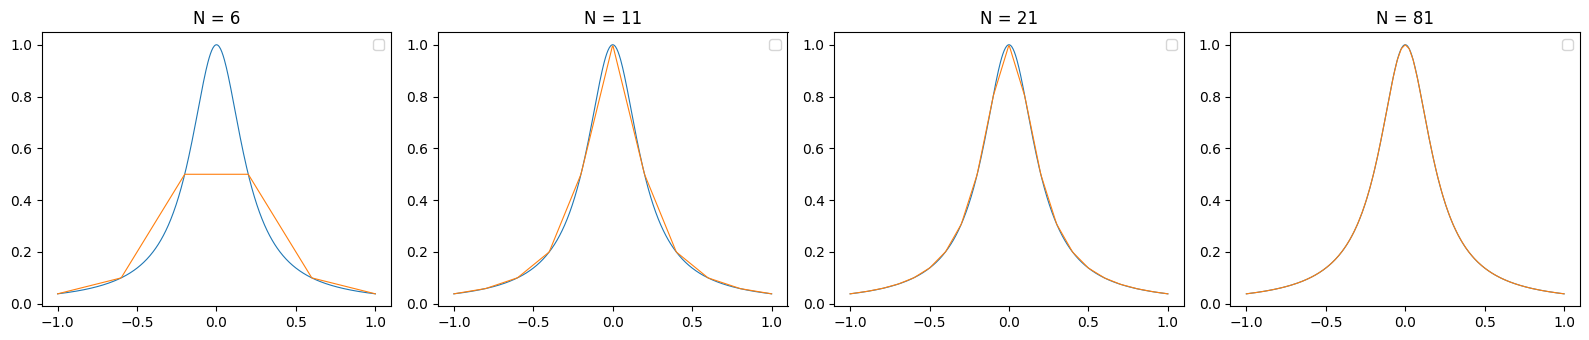
\includegraphics[width=0.9\linewidth]{A1.png}
\end{figure}

三次自然样条:

\begin{figure}[H]
  \centering
  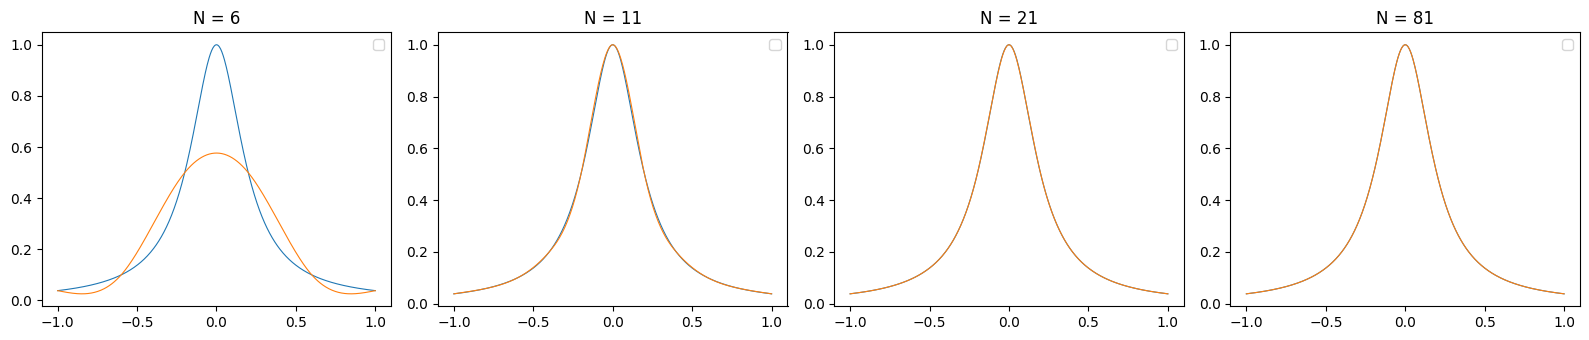
\includegraphics[width=0.9\linewidth]{A3.png}
\end{figure}

三次完全样条:

\begin{figure}[H]
  \centering
  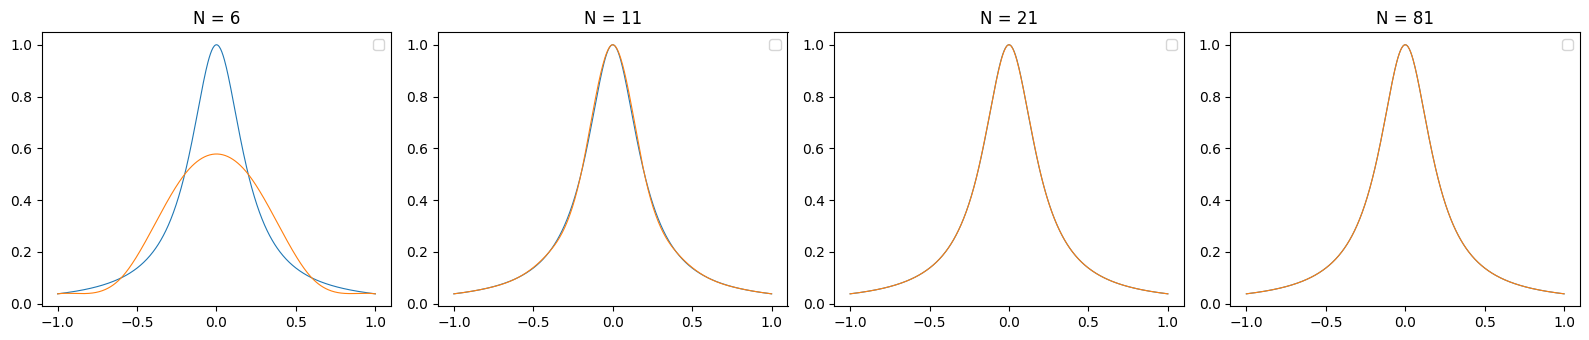
\includegraphics[width=0.9\linewidth]{A2.png}
\end{figure}

三次端点处二阶导给定样条:

\begin{figure}[H]
  \centering
  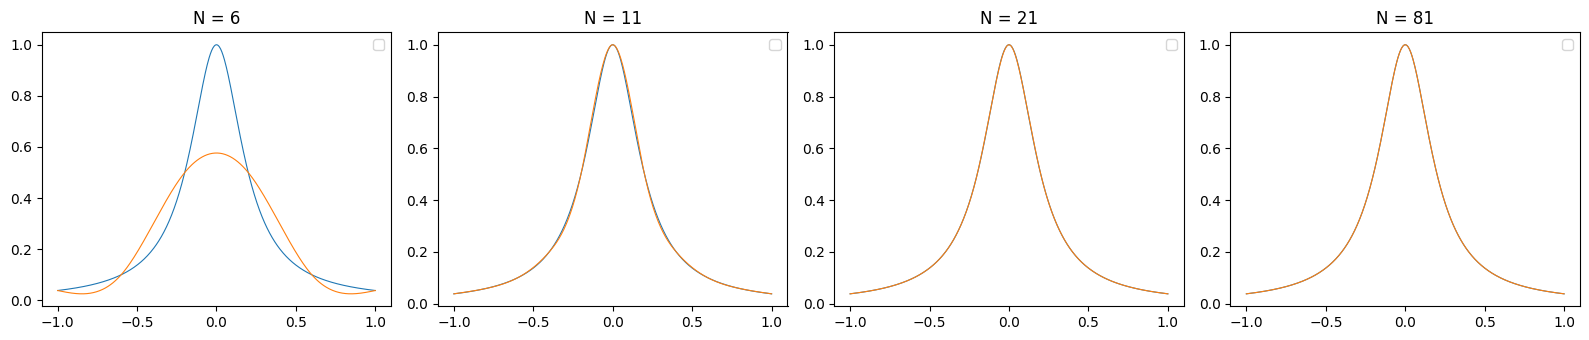
\includegraphics[width=0.9\linewidth]{A4.png}
\end{figure}

使用每一个插值区间的中点处误差组成的误差向量的无穷范数作为误差指标。

误差关于 $N$ 的变化如下所示:

\begin{figure}[H]
  \centering
  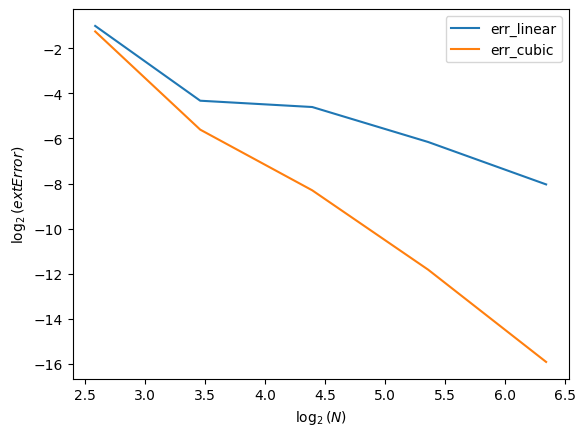
\includegraphics[width=0.5\linewidth]{A5.png}
\end{figure}

由图可以看出,$N$ 越大误差越小,根据斜率可以得到线性样条为2阶收敛,三次样条为4阶收敛。

\subsection{B 样条 $\SBB_n^{n-1}$(Bonus)}

求解函数:
\[f(x) = \dfrac{1}{1+x^2}\]
\[f'(x) = \dfrac{-2x}{(1+x^2)^2}\]
\[f''(x) = \dfrac{-2+6x^2}{(1+x^2)^3}\]

对于1,3,5,7次样条进行测试,采用非均匀的输入点,输入点以及边界条件见 \lstinline{data/BForm.json}。

得到结果如下(输出结果见 \lstinline{res/B.txt}):

\begin{figure}[H]
  \centering
  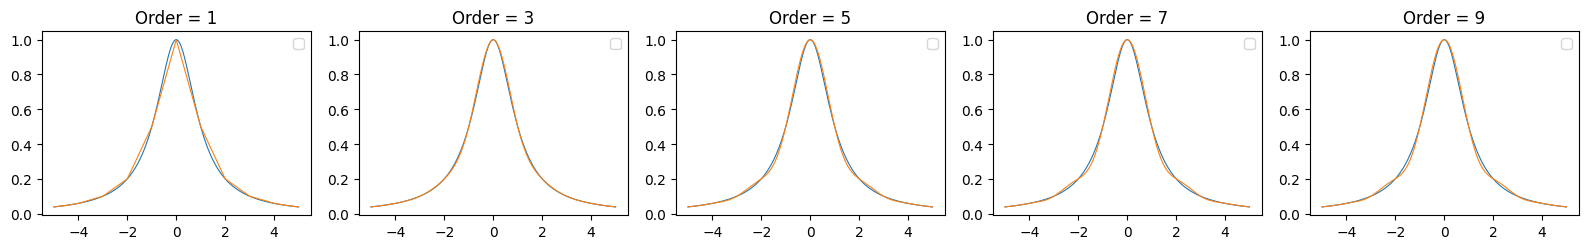
\includegraphics[width=0.9\linewidth]{B1.png}
\end{figure}

这里可以发现5,7,9阶样条的拟合效果不如3阶样条来的好,
这是因为 $n$ 阶样条的误差上界与 $n+1$ 阶导数的最大值有关,
而本题中选取的输入点的间隔较大(输入点数比较少),此时高阶导数值的增长
主导了误差上界的变化,导致高阶样条的拟合效果不够好。
需要进一步增加输入点数,才可以使得高阶样条的拟合效果变好。


\subsection{C. Cubic/Quadratic Cardinal B 样条}

求解函数同 B。

对于 Cubic Cardinal B 样条,
输入点为 $-5, -4, \cdots, 4, 5$。

得到结果如下(输出结果见 \lstinline{res/C.txt}):

对于 Quadratic Cardinal B 样条, 
输入点为 $-4.5, -3.5, \cdots, 3.5, 4.5$,$L = -5, R = 5$。
得到结果如下:

\begin{figure}[H]
  \centering
  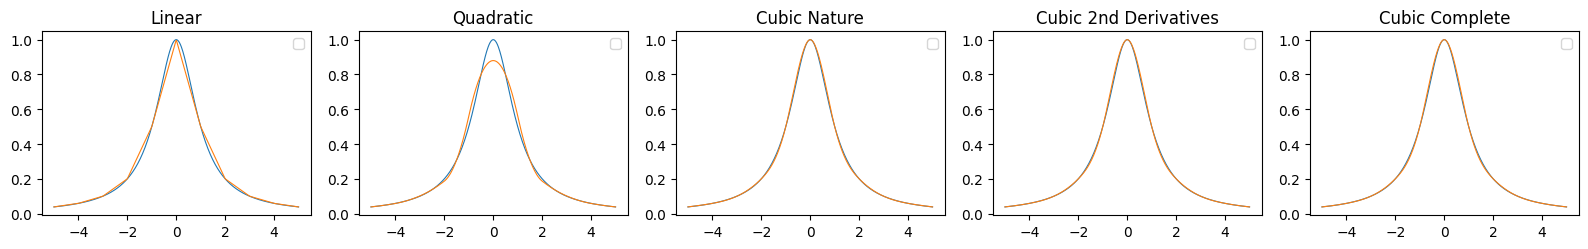
\includegraphics[width=0.9\linewidth]{C1.png}
\end{figure}

二次样条因为没有取到原点作为节点,因此在0附近的拟合误差明显。


\subsection{D. 误差分析}

求解部分位于 \lstinline{Problem-C.cpp}。

令 $E_s(x) = | s(x) - f(x) |$,
对于 C 题中的两种样条,分别计算 $E_s(x)$ 在
$-3.5, -3, \cdots, 3, 3.5$ 处的误差。

得到结果如下(输出结果见 \lstinline{res/C.txt}):

\begin{table}[h]
  \centering
  \begin{tabular}{|c|c|c|c|c|c|}
  \hline
  \textbf{Error Points} & \textbf{Linear} & \textbf{Quadratic} & \textbf{Nature} & \textbf{2nd Derivatives} & \textbf{Complete} \\
  \hline
  -3.5 & 0.00394007 & 1.38778e-17 & 0.000789971 & 0.00068675 & 0.000669568 \\
  -3 & 0 & 0.00141838 & 1.11022e-16 & 9.71445e-17 & 1.11022e-16 \\
  -2.5 & 0.012069 & 0 & 0.00214999 & 0.00212237 & 0.00211777 \\
  -2 & 0 & 0.0132731 & 9.71445e-16 & 9.71445e-16 & 9.71445e-16 \\
  -1.5 & 0.0423077 & 0 & 0.0103452 & 0.0103379 & 0.0103367 \\
  -1 & 0 & 0.0607133 & 1.54876e-14 & 1.54876e-14 & 1.54321e-14 \\
  -0.5 & 0.05 & 0 & 0.0205306 & 0.0205291 & 0.0205289 \\
  0 & 0 & 0.120238 & 4.21885e-15 & 4.10783e-15 & 4.32987e-15 \\
  0.5 & 0.05 & 1.11022e-16 & 0.0205306 & 0.0205291 & 0.0205289 \\
  1 & 0 & 0.0607133 & 6.66134e-16 & 6.66134e-16 & 5.55112e-16 \\
  1.5 & 0.0423077 & 0 & 0.0103452 & 0.0103379 & 0.0103367 \\
  2 & 0 & 0.0132731 & 5.4956e-15 & 5.4956e-15 & 5.4956e-15 \\
  2.5 & 0.012069 & 0 & 0.00214999 & 0.00212237 & 0.00211777 \\
  3 & 0 & 0.00141838 & 2.26208e-15 & 2.27596e-15 & 2.28983e-15 \\
  3.5 & 0.00394007 & 1.38778e-17 & 0.000789971 & 0.00068675 & 0.000669568 \\
  \hline
  \end{tabular}
  \end{table}

  可以发现,对于1次、3次样条,在整点处的误差接近机器精度,
  这是因为这些点是样条的结点,
  而对于2次样条,在半整点处的误差接近机器精度,
  这是因为2次样条采用半整点作为结点。

  可以发现,二次样条在零附近的误差很大,在-3,3处的误差也达到了 1e-3 级别,
  相比之下三次样条的拟合效果好很多。


\subsection{E. 心形曲线拟合}

曲线方程
\[x^2 + \left(\dfrac32 y - \sqrt{|x|}\right)^2 = 3\]

利用极坐标转化为参数方程
\[\begin{cases}x(t) = \sqrt{3} \sin t \\
  y(t) = \dfrac23 \left(\sqrt{3} \cos t + \sqrt{\sqrt{3} |\sin t|}\right)
\end{cases}\]

考虑到 $t = 0, t = \pi$ 处为曲线的关键节点,
考虑取该两个点,再分别在 $t\in[0, \pi], t\in[\pi, 2\pi]$ 的内部,
根据累积弧长均匀地找到 $\dfrac{N-2}2$ 个点。

具体的,计算出曲线总弧长 $L$,分别在累积弧长为 $k\dfrac{L}{n}$ 的位置取点,
取点过程需要用到二分法和自适应辛普森积分。
本题输入数据的生成器见 \lstinline{Problem-E-genData.cpp}。

使用自然,完全,端点处二阶导给定的 $\SBB_3^2$ B 样条进行求解。

得到结果如下(输出结果见 \lstinline{res/E.txt}):

\begin{figure}[H]
  \centering
  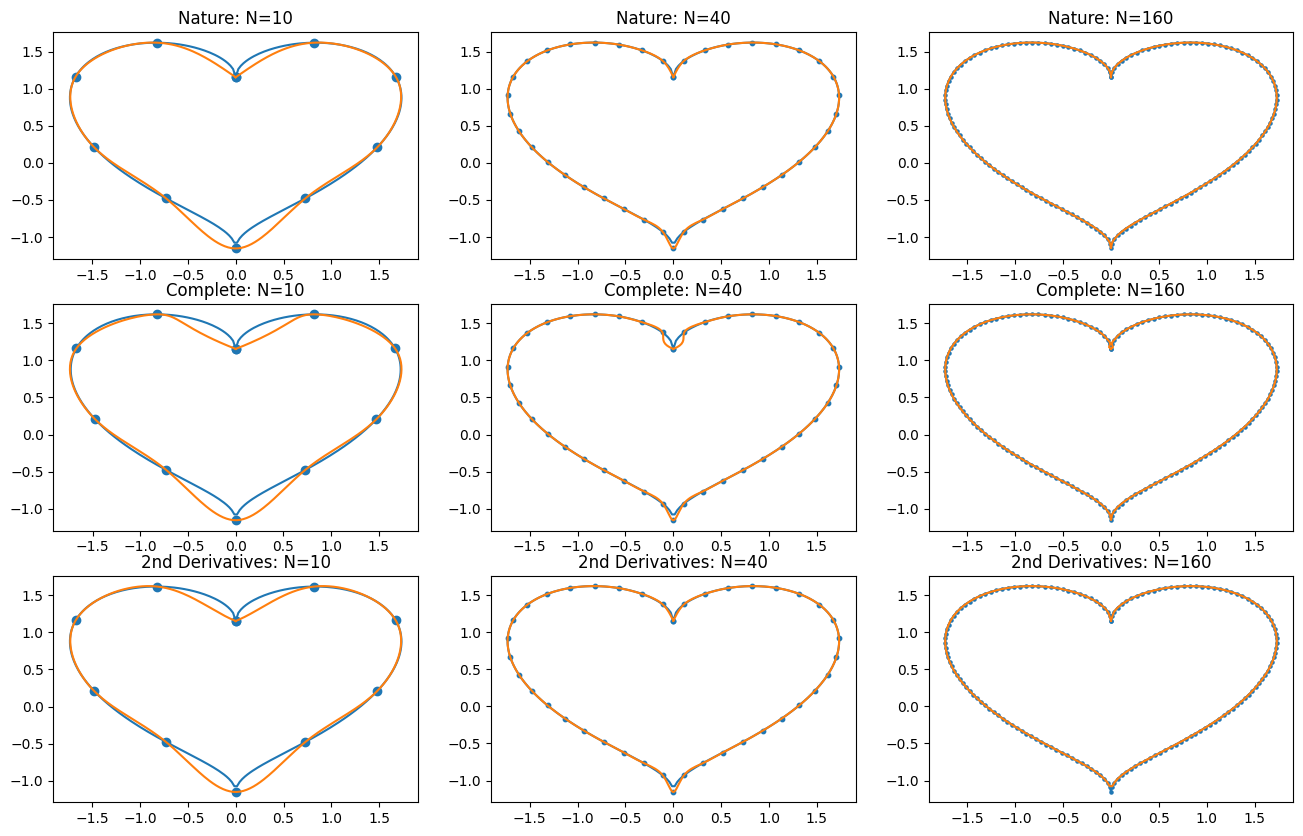
\includegraphics[width=0.9\linewidth]{E1.png}
\end{figure}

在 $N=10$ 的时候,三种边界条件的样条都没有办法很好地拟合出 $t=\pi$ 的图像,
而在 $N=40,N=160$ 的时候,拟合效果明显变好。
完全样条因为无法给定确切的边界点的一阶导值,导致在 $N=10, N=40$ 时候均无法
拟合出心形上部的转角。若采用自然样条,在 $N=40$ 时既可以拟合出效果较佳的图像。


对于边界条件,由于本题 $Y(t)$ 的在端点处的一阶导和二阶导都不存在,
并且由于需要转化为累积弧长为参数的方程,
完全样条和端点处二阶导给定的样条的在给边值条件的时候比较困难。
我认为比较好的边值条件(对于三次样条)应当是自然样条与周期样条(未实现)。


\subsection{误差收敛阶测试(Bonus)}

测试代码见 \lstinline{Convergence-analysis.cpp}。

对于 ppForm 线性样条、完全三次样条,
B Form 线性样条,二次样条,完全三次样条,四次样条,五次样条
取总点数为 $10, 12, 14, \cdots, 100$。
分别计算了误差的无穷范数和二范数。

得到结果如下(输出结果见 \lstinline{res/als.txt}):

\begin{figure}[H]
  \centering
  \begin{subfigure}[b]{0.45\textwidth}
      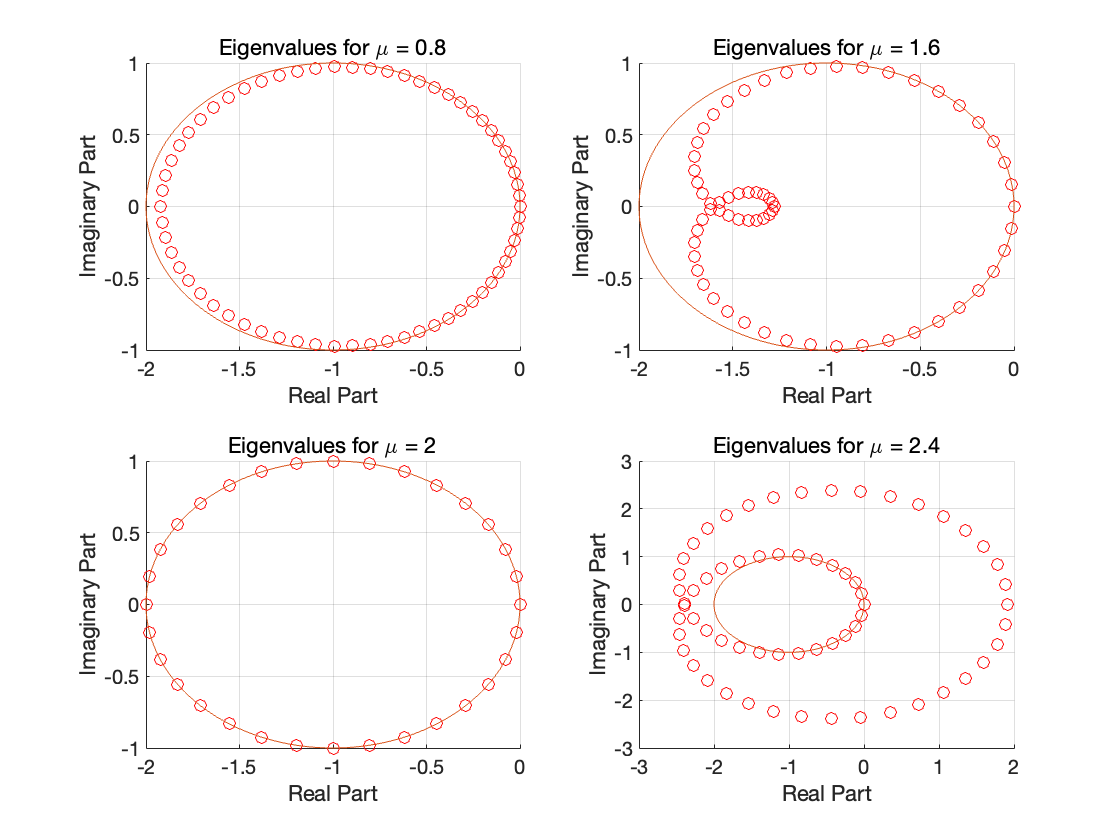
\includegraphics[width=\textwidth]{1.png}
  \end{subfigure}
  \hfill
  \begin{subfigure}[b]{0.45\textwidth}
    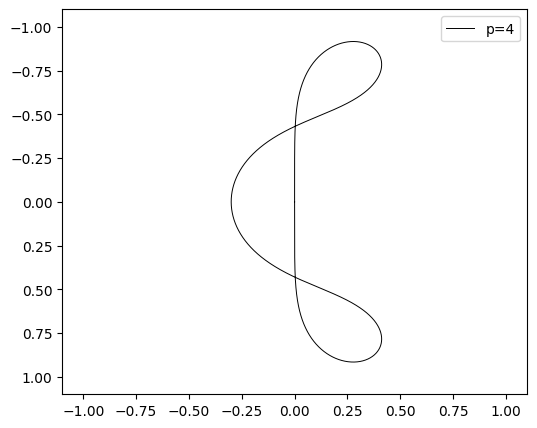
\includegraphics[width=\textwidth]{2.png}
\end{subfigure}
  
  \medskip
  
  \begin{subfigure}[b]{0.45\textwidth}
    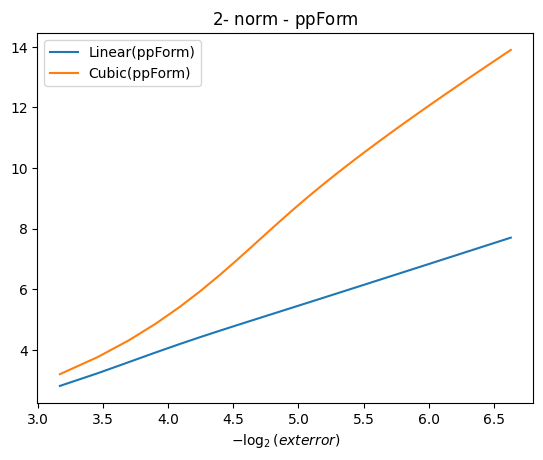
\includegraphics[width=\textwidth]{3.png}
\end{subfigure}
  \hfill
  \begin{subfigure}[b]{0.45\textwidth}
    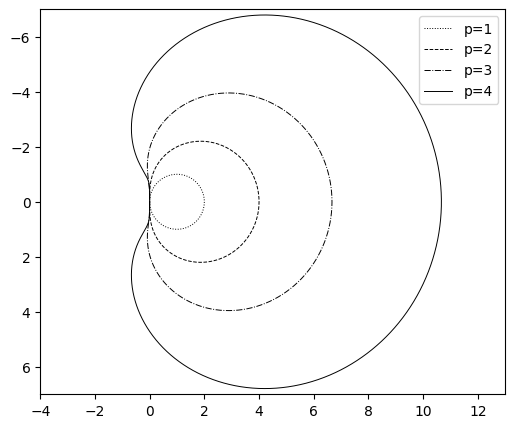
\includegraphics[width=\textwidth]{4.png}
\end{subfigure}
\end{figure}


对于 ppForm,线性样条为 2 阶收敛,三次样条为四阶收敛。

对于 B Form,可以发现高次样条的收敛阶更高。$n$ 次样条接近 $n+1$ 阶收敛。

由于 二次,四次样条在提供边值条件时,左右提供的条件不对称,导致其在 $h$ 较大的时候会出现
振荡,因此收敛性质收到影响。比如下图为 B Form $\SBB_2^1$ 的图像:

\begin{figure}[H]
  \centering
  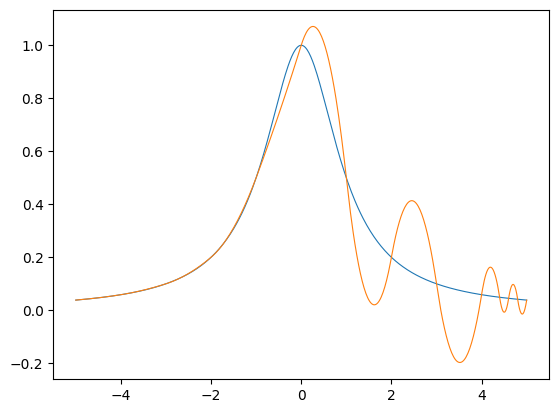
\includegraphics[width=0.45\linewidth]{B2.png}
\end{figure}


\nocite{*}
\printbibliography[heading=bibintoc, title=\ebibname]

% \appendix
% % \appendixpage
% \addappheadtotoc

\end{document}
